%
% File twocolumn.tex
%%
%% Based on the style files for *SEM-2014, which were, in turn,
%% Based on the style files for COLING-2014, which were, in turn,
%% Based on the style files for ACL-2014, which were, in turn,
%% Based on the style files for ACL-2013, which were, in turn,
%% Based on the style files for ACL-2012, which were, in turn,
%% based on the style files for ACL-2011, which were, in turn,
%% based on the style files for ACL-2010, which were, in turn,
%% based on the style files for ACL-IJCNLP-2009, which were, in turn,
%% based on the style files for EACL-2009 and IJCNLP-2008...

%% Based on the style files for EACL 2006 by
%%e.agirre@ehu.es or Sergi.Balari@uab.es
%% and that of ACL 08 by Joakim Nivre and Noah Smith

\documentclass[11pt]{article}
\usepackage{semeval2014}
\usepackage{times}
\usepackage{latexsym}
\usepackage{color}
\usepackage[usenames,dvipsnames,svgnames,table]{xcolor}
\usepackage{amsmath}
\usepackage{bm}
\usepackage{amssymb}
\usepackage{graphicx}
\usepackage{enumitem}
\usepackage{multirow}
\usepackage{tabularx}
\usepackage{framed}
\usepackage{url}
\usepackage{footnote}
\usepackage{microtype}
\usepackage[small,bf,skip=5pt]{caption}

\setitemize{noitemsep,topsep=10pt,parsep=0pt,partopsep=0pt}
\setenumerate{noitemsep,topsep=10pt,parsep=0pt,partopsep=0pt}

%\setlength\titlebox{5cm}

% You can expand the titlebox if you need extra space
% to show all the authors. Please do not make the titlebox
% smaller than 5cm (the original size); we will check this
% in the camera-ready version and ask you to change it back.

\newcommand{\wsname}{SemEval-2014}
\newcommand{\submissionpage}{\url{http://alt.qcri.org/semeval2014/index.php?id=cfp}}
\newcommand{\filename}{semeval2014}
\newcommand{\contact}{pnakov qf.org.qa}

\renewcommand\floatpagefraction{.9}
\renewcommand\topfraction{.9}
\renewcommand\bottomfraction{.9}
\renewcommand\textfraction{.1}   


\definecolor{myblue}{rgb}{0,0.1,0.6}
\definecolor{mygreen}{rgb}{0,0.3,0.1}
\usepackage[colorlinks=true,linkcolor=black,citecolor=mygreen,urlcolor=myblue]{hyperref}
\newcommand{\transpose}{^\mathsf{T}}
\DeclareMathOperator*{\argmax}{arg\,max}

\newcommand{\bocomment}[1]{\textcolor{Bittersweet}{[#1 -BTO]}}
\newcommand{\sam}[1]{\textcolor{blue}{[#1 -SMT]}}
\newcommand{\nas}[1]{\textcolor{red}{[#1 -NAS]}}
\newcommand{\jmf}[1]{\textcolor{orange}{[#1 -JMF]}}
\newcommand{\jdcomment}[1]{\textcolor{NavyBlue}{[#1 -JDD]}}

 \renewcommand{\bocomment}[1]{}
 \renewcommand{\sam}[1]{}
 \renewcommand{\nas}[1]{}
 \renewcommand{\jmf}[1]{}
 \renewcommand{\jdcomment}[1]{}


% turn off for submission, but on for a more tech report-y version.
% \newcommand{\codenote}[1]{\textcolor{PineGreen}{[#1]}}
\newcommand{\codenote}[1]{}
% \newcommand{\logitedge}{\textsc{IndepEdge}}
\newcommand{\logitedge}{\textsc{LogisticEdge}}
\newcommand{\svmedge}{\textsc{SvmEdge}}
\newcommand{\noedge}{\textsc{NoEdge}}

% saves only a little bit of space. might need tweaking to save more.
\newenvironment{itemizesquish}{\begin{list}{\labelitemi}{\setlength{\itemsep}{-0.1em}\setlength{\labelwidth}{1em}\setlength{\leftmargin}{\labelwidth}\addtolength{\leftmargin}{\labelsep}}}{\end{list}}

\expandafter\def\expandafter\normalsize\expandafter{%
    \normalsize
    \setlength\abovedisplayskip{9pt}
    \setlength\belowdisplayskip{9pt}
    \setlength\abovedisplayshortskip{9pt}
    \setlength\belowdisplayshortskip{9pt}
}
% \renewcommand{\baselinestretch}{0.95}

\hyphenation{SemEval}
\hyphenation{ana-ly-sis}
\hyphenation{Logistic-Edge}
\hyphenation{Svm-Edge}


\title{CMU-ARK: Arc-Factored, Discriminative Semantic Dependency Parsing}

\author{
	Sam Thomson \quad
	Brendan O'Connor \quad
	Jeff Flanigan \quad
	David Bamman \quad  \\
	\bf{Jesse Dodge \quad
	Swabha Swayamdipta \quad
	Nathan Schneider \quad
	Chris Dyer \quad
	Noah A.~Smith} \\
  Language Technologies Institute \\
  Carnegie Mellon University \\
  Pittsburgh, PA 15213, USA \\
  {\tt\{sthomson,brenocon,jflanigan,dbamman,jessed,}\\
   \tt{swabha,nschneid,cdyer,nasmith\}@cs.cmu.edu}
}

\date{}

\begin{document}
\maketitle

\begin{abstract}
We present an arc-factored statistical model for
semantic dependency parsing, as defined by the SemEval 2014 Shared
Task 8 on
Broad-Coverage Semantic Dependency Parsing.    Our entry in the open
track placed second in the competition.
\end{abstract}



\section{Introduction}

The task of broad coverage semantic dependency parsing aims to provide a
shallow semantic analysis of text not limited to a specific domain.
As distinct from deeper semantic analysis (e.g., parsing to a full
lambda-calculus logical form), shallow semantic parsing captures relationships
between pairs of words or concepts in a sentence, and has wide application for
information extraction, knowledge base population, and question answering (among others).
%The SemEval 2014 Shared Task 8 on Broad-Coverage Semantic Dependency
%Parsing \cite{oepens_broad_2014} includes three different semantic
%formalisms (\S\ref{s:formalisms}), which encourages finding features and methods
%that are broadly applicable to semantic parsing, and discourages optimization
%toward a single semantic representation.
%By diversifying the representations, we better tackle the broader task of
%semantic analysis itself.

We present here two systems that produce semantic dependency parses in the three formalisms of the SemEval 2014 Shared Task 8 on Broad-Coverage Semantic Dependency
Parsing \cite{oepens_broad_2014}.  These systems generate parses by extracting
features for each potential dependency arc and learning a statistical model to
discriminate between good arcs and bad;
the first treats each labeled edge decision as an independent multiclass
logistic regression (\S\ref{s:logitedge}), while the second predicts arcs
as part of a graph-based structured support vector machine (\S\ref{s:graphparser}).
Common to both models is a rich set of features on arcs, described in
\S\ref{s:edgefeatures}.  We include a discussion of features found to
have no discernable effect, or negative effect, during development (\S\ref{s:badfeatures}).

Our system placed second in the open track of the Broad-Coverage Semantic
Dependency Parsing task (in which output from syntactic parsers and other outside resources \emph{can} be used).
We present our results in \S\ref{s:evaluation}.



\section{Formalisms} \label{s:formalisms}
The Shared Task 8 dataset consists of annotations of the Penn Treebank in
three different semantic dependency formalisms.
%The organizers of Shared Task 8 provided a corpus of English news text
%drawn from the Penn Treebank, annotated according to three different semantic dependency formalisms.
\emph{DM} is derived from LinGO English Resource Grammar (ERG)
annotations in DeepBank \cite{flickinger_deepbank_2012}.
\emph{PAS} is derived from the Enju HPSG treebank using the
conversion rules of \newcite{miyao_corpus_oriented_2004}.
\emph{PCEDT} is derived from the tectogrammatical layer of the
Prague Czech-English Dependency Treebank \cite{hajic_building_1998}.
See Figure~\ref{fig:formalisms} for an example.
\begin{figure}
	\centering
		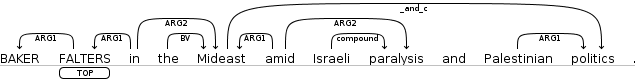
\includegraphics[width=.5\textwidth]{fig/example_dm} \\
		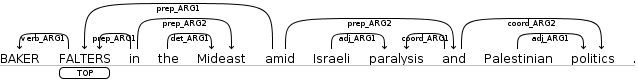
\includegraphics[width=.5\textwidth]{fig/example_pas} \\
		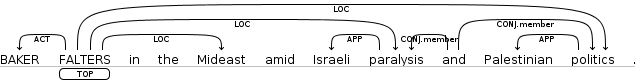
\includegraphics[width=.5\textwidth]{fig/example_pcedt}
	\caption{Example annotations for \emph{DM} (top), \emph{PAS}
          (middle), and \emph{PCEDT} (bottom).}
	\label{fig:formalisms}
\end{figure}

The three formalisms come from very different linguistic theories, but all
are represented as labeled directed graphs, with words as vertices, and
all have ``top'' annotations, corresponding roughly to the
semantic focus of the sentence.  
(A ``top'' need not be a root of the
graph.)
This allows us to use the same machinery (\S\ref{s:models}) for
training and testing statistical models for the three formalisms.
\sam{Stats about \% multiple roots, \% multiple tops, \% tree, \% acyclic}



\section{Models} \label{s:models}

We treat the problem as a three-stage pipeline.
The first stage prunes words by predicting whether they have any incoming or
outgoing edges at all (\S\ref{s:singleton_model}); 
if a word does not, then it is not 
considered for any attachments in later stages.
The second stage predicts where edges are
present, and their labels (\S\ref{s:edge_model}).
The third stage predicts whether a predicate word is a \emph{top} or not
(\S\ref{s:top_model}).
Formalisms sometimes annotate more than one ``top'' per sentence, but we
found that we achieve the best performance on all formalisms by predicting only
the one best-scoring ``top'' under the model.
\bocomment{Singleton pruning does not matter for LogitEdge.  It doesn't affect accuracy, I'm pretty sure.  But it is essential for the graph model.}



\subsection{Singleton Classification} \label{s:singleton_model}

For each formalism, we train a classifier to recognize \emph{singletons},
nodes that have no parents or children.
(For example, punctuation tokens are often singletons.)
This makes the system faster without affecting accuracy.
For singleton prediction, we use a token-level logistic regression
classifier, with features including
the word, its lemma, and its
part-of-speech tag.
If the classifier predicts a probability of 99\% or higher 
the token is pruned; this removes around 10\% of tokens.
(The classifier performs differently on different formalisms;
on \emph{PAS} it has perfect accuracy, 
while on
\emph{DM} and \emph{PCEDT} accuracy is in the mid-90's.)




\subsection{Edge Prediction} \label{s:edge_model}

In the second stage of the pipeline, we predict the set of labeled directed
edges in the graph.
We use the same set of edge-factored features (\S\ref{s:features}) in two
alternative models: an edge-independent multiclass logistic
regression model (\logitedge, \S\ref{s:logitedge}); and a structured SVM 
\cite{taskar_max_2003,tsochantaridis_support_2004} that enforces 
\emph{determinism} constraints which allow a word to
have at most one outgoing edge with the
same label (\svmedge, \S\ref{s:graphparser}).
For each formalism, we trained both models with varying features enabled and
hyperparameter settings and submitted the configuration that produced the best
labeled $F_1$ on the development set.
For \emph{DM} and \emph{PCEDT}, this was \logitedge;
for \emph{PAS}, this was \svmedge.
We report results only for the submitted configurations, with different features
enabled.
Due to time constraints, full hyperparameter sweeps and comparable feature sweeps were not possible.


\subsubsection{\logitedge\ Parser}
\label{s:logitedge}


\codenote{LRParser.java}

The \logitedge\ model considers only token index pairs $(i, j)$ where %that are
% within 10 tokens of each other (i.e.~
$|i-j| \leq 10$, $i \ne j$, and both $t_i$ and
$t_j$ have been predicted to be non-singletons by the first stage.
% In other words, edges with more than 9 tokens between its two endpoints are not
% considered.
Although this prunes some gold edges, among the formalisms,
95\%--97\% of all gold edges are between tokens of distance 10 or less.
Both directions $i \rightarrow j$ and $j \rightarrow
i$ are considered between every pair.

%\noindent
Let $L$ be the set of $K+1$ possible output labels: the formalism's original $K$
edge labels, plus the additional label \noedge, which indicates that no edge
exists from $i$ to $j$.
The model treats every pair of token indices $(i, j)$ as an
independent multiclass logistic regression over output space $L$:

Let $x$ be an input sentence.
For candidate parent index $i$, child index $j$, and edge label $\ell$, we
extract a feature vector $\bm{f}(x, i, j, \ell)$, where $\ell$ is conjoined with
every feature described in \S\ref{s:features}.
The multiclass logistic regression model defines a distribution over $L$,
parametrized by weights $\bm\phi$:
\[
  P(\ell\mid\bm\phi,x, i,j)  = \frac{
  	\exp\{\bm\phi \cdot \bm{f}(x, i, j, \ell)\}
  } {
  	\sum_{\ell^\prime \in L} {
  		\exp\{\bm\phi \cdot \bm{f}(x, i, j, \ell^\prime)\}
  	}
  }
\]

\noindent
$\bm\phi$ is learned by minimizing total negative log-likelihood of the above
(with weighting; see below), plus $\ell_2$ regularization.
AdaGrad \cite{duchi_adaptive_2011} is used for optimization.
This seemed to optimize faster than L-BFGS \cite{Liu1989LBFGS}, at least for earlier
iterations, though we did no systematic comparison. Stochastic gradient steps
are applied one at a time from individual examples, and a gradient step for the
regularizer is applied once per epoch.

The output labels have a class imbalance; in all three formalisms, there
are many more $\noedge$ examples than true edge examples.
\sam{If we get these numbers, it would be nicer to quantify, and say something
like ``In the FFF formalism, the training set (\S\ref{s:evaluation}) contains NNN
candidate edges (pairs of tokens with length between 1 and 10 inclusive), and NNN actual (non-null) edges.''}
We improved $F_1$ performance by
downweighting $\noedge$ examples through a weighted log-likelihood objective,
$\sum_{i,j} \sum_\ell w_\ell \log P(\ell \mid \bm\phi, x, i, j)$, 
with $w_{\noedge}=0.3$ (selected on development set)
and $w_{\ell} = 1$ otherwise.

% 0.4

% Besides the edge logistic regression system, there were both pre- and post-processing steps.

% \textbf{Preprocessing:}
% \bocomment{TODO need to check how much preproc was used for this.  Was singleton pruning turned on?  It looks like we commented out the prune features in LRParser.java.  But singleton pruning might have been turned on.}

% \textbf{Decoding and postprocessing:}
\noindent
\textbf{Decoding:} \codenote{MyGraph::decodeEdgeProbsToGraph()}
To predict a graph structure at test-time for a new sentence,
the most likely edge label is predicted for every candidate $(i, j)$ pair of
unpruned tokens.
If an edge is predicted for both directions for a single $(i,j)$
pair, only the edge with the higher score is chosen.
(There are no such bidirectional edges in the training data.)
This post-processing actually did not improve accuracy on \emph{DM} or \emph{PCEDT};
it did improve \emph{PAS} by $\approx0.2\%$ absolute $F_1$, but we did not submit \logitedge\ for \emph{PAS}.
\codenote{\url{https://github.com/Noahs-ARK/semeval-2014/pull/21}}


\subsubsection{\svmedge~Parser}
\label{s:graphparser}



In the \svmedge~model, we use a structured SVM
with a determinism constraint.
This constraint ensures that each word token has at most one outgoing edge for
each label in a set of deterministic labels $L_d$.
For example, in \emph{DM} a predicate never has more than one child with edge
label ``ARG1.''
 $L_d$ was chosen to be the set of edges that were $> 99.9\%$
deterministic in the training data.\footnote{
By this we mean that of the nodes that have at least one
outgoing $\ell$ edge, $99.9\%$ of them have only one outgoing $\ell$ edge.
For \emph{DM}, $L_d=L \setminus$\{``\_and\_c,'' ``\_or\_c,'' ``\_then\_c,''
``loc,'' ``mwe,'' ``subord''\};
for \emph{PAS}, $L_d = L$;
and for \emph{PCEDT}, $L_d=$\{``DPHR,'' ``INTF,''  ``VOCAT''\}.}
%We found this contraint improved the $F_1$-score for the
%\emph{PAS} formalism only.

Consider the fully dense graph of all edges between all words predicted
as not singletons by the singleton classifier \S\ref{s:singleton_model} (in all
directions with all possible labels). Unlike \logitedge, the label set $L$ does
not include an explicit \textsc{NoEdge} label.
If $\bm\psi$ denotes the model
weights, and $\bm{f}$ denotes the features, then an edge from $i$ to $j$ with
label $\ell$ in the dense graph has a weight $c(i,j,\ell)$ assigned to it using the linear
scoring function $c(i,j,\ell) = \bm\psi \cdot \bm{f}(x,i,j,\ell)$.

\noindent
\textbf{Decoding:} For each node and each label $\ell$, if $\ell \in L_d$, the
decoder adds the highest scoring outgoing edge, if its weight is positive.
For $\ell \not\in L_d$, every outgoing edge with positive weight is added.
This procedure is guaranteed to find the highest scoring subgraph (largest sum
of edge weights) of the dense graph subject to the determinism constraints.
Its runtime is $O(n^2)$.



The model weights are trained using the structured SVM loss.  If $x$
is a sentence and $y$ is a graph over that sentence, let the features 
be denoted $\bm{f}(x,y) = \sum_{(i,j,\ell) \in y}
\bm{f}(x, i,j,\ell)$.  The SVM loss for each training example $(x_i, y_i)$ is:
\begin{multline*}
-\bm\psi^\top \bm{f}(x_i,y_i) + \max_{y} \bm\psi^\top \bm{f}(x_i,y) +
\mathit{cost}(y,y_i)
\end{multline*}
where $\mathit{cost}(y,y_i) = \alpha |y\setminus y_i| +
\beta |y_i\setminus y|$.
$\alpha$ and $\beta$ trade off between precision and recall for the
edges \cite{gimpel_softmax-margin_2010}.
The loss is minimized with AdaGrad
using early-stopping on a development set. % Tops are predicted using the
%top prediction model \S\ref{s:top_model}.


\subsubsection{Edge Features}
\label{s:edgefeatures}

\label{s:features}

\sam{would be nice to cite where we stole these features from, where applicable}
Table~\ref{table:edgefeatures} describes the features we used for predicting
edges.
These features were computed over an edge $e$ with parent token $s$ at
index $i$ and child token $t$ at index $j$. 
Unless otherwise stated, each feature template listed has an indicator
feature that fires for each value it can take on.  For the submitted results,
\logitedge~uses all features except Dependency Path v2, POS Path, and Distance
Thresholds, and \svmedge~uses all features except Dependency
Path v1.  This was due to \svmedge~being faster to
train than \logitedge~when including POS Path features, and due to time constraints for the submission we were unable to retrain
\logitedge~with these features.

\renewcommand{\floatpagefraction}{0.8}
\begin{table}
\begin{framed}
\begin{small}
%\textbf{Bias:} Always fires.

\textbf{Tokens:} The tokens $s$ and $t$ themselves.

\textbf{Lemmas:} Lemmas of $s$ and $t$.

\textbf{POS tags:} Part of speech tags of $s$ and $t$.

\textbf{Linear Order:} Fires if $i < j$.

\textbf{Linear Distance:} $i - j$.

\textbf{Dependency Path v1 (\logitedge~only):} The concatenation of all POS
tags and arc labels on the labeled path in the syntactic dependency tree from $s$ to
$t$.  Conjoined with $s$, with $t$, and without either.

\textbf{Dependency Path v2 (\svmedge~only):}
Same as Dependency Path v1, but with the lemma of $s$ or $t$ instead of the
word, and substituting the token for any ``IN'' POS tag.

\textbf{Up/Down Dependency Path:} The sequence of upward and
	downward moves needed to get from $s$ to $t$ in the syntactic dependency
	tree.

\textbf{Up/Down/Left/Right Dependency Path:} The unlabeled path through
	the syntactic dependency tree from $s$ to $t$, annotated with whether the each
	step through the tree was up or down, and whether it was to the right or left
	in the sentence.

\textbf{Is Parent:} Fires if  $s$ is the parent of $t$ in the syntactic
	dependency parse.

\textbf{Dependency Path Length:} Distance between $s$ and $t$ in the
	syntactic dependency parse.

\textbf{POS Context:} Concatenated POS tags of tokens at $i-1$, $i$,
	$i+1$, $j-1$, $j$, and $j+1$. Concatenated POS tags of tokens at $i-1, i, j-1$,
	and $j$. Concatenated POS tags of tokens at $i, i+1, j$, and $j+1$.

\textbf{Subcategorization Sequence:} 
	The sequence of dependency arc labels out of $s$, ordered by the index of the
	child.
	Distinguish left children from right children.
	If $t$ is a direct child of $s$, distinguish its arc label with a ``+''.
	Conjoin this sequence with the POS tag of $s$.

\textbf{Subcategorization Sequence with POS:} As above, but add the
	POS tag of each child to its arc label.

\textbf{POS Path (\svmedge~only):}
Concatenated POS tags between and including $i$ and $j$.
Conjoined with head lemma, with dependent lemma, and without either.


\textbf{Distance Thresholds (\svmedge~only):}
Fires for every integer between $1$ and $\lfloor \log(|i-j|+1)/\log(1.39)
\rfloor$ inclusive,
e.g.~$\{1,2,3,5,7,10,\ldots\}$.

\end{small}
\end{framed}
\caption{Features used in edge prediction}
\label{table:edgefeatures}
\end{table}





\subsubsection{Feature Hashing}

%\bocomment{ALTERNATE VERSION TO SAVE SPACE:
  The biggest memory usage was in the map from
  feature names to integer indices during feature extraction.
  For experimental expedience, we
  implemented multitask feature hashing
  \cite{weinberger_feature_2009}, which hashes feature names to indices, under
  the theory that errors due to collisions tend to cancel.  No
  drop in accuracy was observed.

% }
% \sam{I think we can get away with this short version}
% %% 7-10 million features (percepts) before label conjunction:
% % cab:~dbamman/semeval/mar3 % wc -l *.model
% %    7518732 mar3_recsplit.dm.model
% %    7038841 mar3_recsplit.pas.model
% %    9939549 mar3_recsplit.pcedt.model
% %   24497122 total

% \codenote{
% \url{https://github.com/Noahs-ARK/semeval-2014/pull/20}
% Code:
%   See use of flag LRParser.useHashing, esp LRParser::perceptNum() 
%   and Model::coefIdx(): hashed values before and after label conjunction.
% }

% \noindent
% For \logitedge, the biggest memory usage was from
% the hash table that implemented
% a map of feature names to integer indices, used during feature extraction.
% Tens of millions of features (before conjunction) resulted in several gigabytes of memory use.  To facilitate more convenient experimentation,
% we eliminated this by using
% multitask feature hashing
% \cite{weinberger_feature_2009},
% which randomly assigns features' numeric indices with a hash function.\footnote{We also tried replacing the hash table with a Patricia Tree, trying several open-source implementations; but they had worse memory usage than a GNU Trove hash table. 
%   \codenote{\url{https://github.com/brendano/myutil/blob/0a5697a7f066c265a75ce1b7bd527feafa683c8a/src/vocabalts/vocabalts_results.txt}}}
% Let $F$ be the space of all feature names (before conjunction with the output label).
% In the usual approach, a hash table is maintained containing a
% one-one onto map from features to integer indices $g: F \rightarrow \{1,\ldots,|F|\}$,
% and each output label has an array of model parameters $\bm\phi^\ell \in \mathbb{R}^{|F|}$,
% which $g(f)$ indices into.
% In the hashing approach, a hash function $h_{\ell}$
% maps feature name to one of $B$ bucket values,
% $h_{\ell} : F \rightarrow \{1, \ldots, B\}$.
% (A different hash function is used for each output label.)
% The model parameters are stored in an array $h_\ell(\bm\phi^\ell) \in \mathbb{R}^{B}$,
% for which an entry is defined as
% \[
%   h_\ell(\bm\phi^\ell)_{b} = 
%   \sum_{\substack{\text{feat} \in F 
%     \\\text{ s.t. } h_\ell(\text{feat})=b}}
%   {\phi^\ell_{\text{feat}}}
% \]
% This is easy to implement:
% array lookups and gradient steps are simply implemented with $h$ instead of $g$, and feature vectors are also stored in a hashed space.
% \cite{weinberger_feature_2009} show that, even with some collisions,
% dot products are approximately preserved with high probability;
% and indeed, we observed no drop in accuracy compared to using an explicit feature map.
% We used a value of $B$ as large as was convenient for memory usage (due only to $h(\phi)$), $B=10^{8}$.
% This is actually higher than $|F|\approx 10^7$, though plenty of collisions still happen: about 9.5\% of features are hashed to a value shared by at least one other feature.

% %% simulation:
% % num buckets count 0: 90484843
% % num buckets count 1: 9046266
% % num collisions: num features that are in a non-singleton bucket: 953734
% %%  average over simulations for last value: 9.518e+05 


\subsection{Top Prediction} \label{s:top_model}

\bocomment{may15 afternoon: The below describes how top pred works in LogitEdge.  Jeff, please confirm this is how you use the topness classifier, or modify appropriately.}\jmf{yes, this is correct for the graph parser}

We trained a separate token-level binary logistic regression to classify
whether a token's node had the ``top'' attribute or not.
At decoding time, all predicted predicates (i.e., nodes where there is at least one outbound edge)
are possible candidates to be ``top'';
the classifier probabilities are evaluated, and the highest-scoring node is
chosen to be ``top.''
\codenote{LogitEdge: MyGraph::decideTops()}
This is suboptimal, since some graphs have multiple tops (in \emph{PCEDT} this is
more common);
but selection rules based on probability thresholds gave worse $F_1$
performance on the dev set. \codenote{\url{https://github.com/Noahs-ARK/semeval-2014/issues/37}}
For a given token $t$ at index $i$, the top classifier's features
included $t$'s POS tag, $i$, those two conjoined, and the depth
of $t$ in the syntactic dependency tree.


\section{Negative Results}
\label{s:badfeatures}

We followed a forward-selection process during feature engineering.
For each potential feature, we tested the current feature set versus the current
feature set plus the new potential feature.
If the new feature did not improve performance, we did not add it.
We list in table \ref{table:negedgefeatures} some of the features which we tested but did not improve
performance.

In order to save time, we ran these feature selection experiments
on a subsample of the training data, for a reduced number of iterations.
These results thus have a 
 strong caveat that the experiments were
not exhaustive.  It may be that some of these features could help under more careful study.

\begin{savenotes}
\begin{table}
\small
\begin{framed}
%\textbf{Bias:} Always fires.

\textbf{Word vectors:} Features derived from 64-dimensional vectors from  \cite{wordVectors}, including the
concatenation, difference, inner product, and element-wise multiplication of the two vectors associated with a parent-child edge. We also trained a random forest\footnote{Using \cite{RandomForest2002}'s \emph{randomForest} R implementation.} on the word vectors (using the vector elements as features to predict the observed semantic label); at test time, the predicted hard labels were incorporated as features.

\textbf{Brown clusters} Features derived from Brown clusters \cite{Brown:1992:CNG:176313.176316}
trained on a large corpus of web data. Parent, child, and conjoined parent-child
edge features from cluster prefixes of length 2, 4, 6, 8, 10, and 12.
Conjunctions of those features with the POS tags of the parent and child tokens.

\textbf{Active/passive:} Active/passive voice feature
(as in \newcite{johansson_dependency-based_2008}) conjoined with both the Linear
Distance features and the Subcategorization Sequence features.
Voice information may already be captured by features from the Stanford
dependency--style parses, which include passivization information in arc labels such as \emph{nsubjpass} and
\emph{auxpass} \cite{Marneffe2008DepColing}.


\textbf{Connectivity constraint:} Enforcing that the graph is connected (ignoring singletons), similar
to \newcite{flanigan-etal:ACL2014}. Almost all semantic dependency graphs are connected (ignoring singletons) in the
training data, but we found that enforcing this constraint caused more edges to
be predicted, significantly hurting performance.

\textbf{Tree constraint:} Enforces that the graph is a tree. Unsurprisingly, we found that enforcing a tree constraint hurt performance.

\end{framed}
\small
\caption{Features and constraints giving negative results.}
\label{table:negedgefeatures}
\end{table}
\end{savenotes}

% For each method outlined below, each dimension of the output vector was used as
% a feature, whose value was the value of the vector along that dimension.
% %As an example, if we concatenated the two vectors into a third vector $V_3$ (as
% %we show in $f_1$), each element of $V_3$ was used as a feature in our model.

% \begin{itemize}
% \item Concatenation:
% $ \left( \begin{smallmatrix} \bm{v_1}\\ \bm{v_2}
% \end{smallmatrix} \right)$
% \item Difference: $\bm{v_1} - \bm{v_2}$.
% \item Dot product: $\bm{v_1} \cdot \bm{v_2}$
% \item Element-wise multiplication: $\bm{v_1} \bigodot \bm{v_2}$
% \end{itemize}
% Unfortunately we saw no improvement from these features.



\section{Experimental Setup}
\label{s:evaluation}

We participated in the Open Track, and used the syntactic dependency parses supplied by the organizers.  Feature engineering was performed on a development set (\S 20), training on \S 00--19.
We evaluate labeled precision (LP), labeled recall (LR), labeled $F_1$ (LF), and
labeled whole-sentence match (LM) on the held-out test data using the
evaluation script provided by the organizers. 
LF was averaged over the formalisms to determine the winning system.
Table~\ref{table:perf} shows our scores.

% CMU:
% DM:
% LP: 0.844641
% LR: 0.834849
% LF: 0.839716
% LM: 0.087537
% 
% 
% PAS:
% LP: 0.907832
% LR: 0.885141
% LF: 0.896343
% LM: 0.260386
% 
% 
% PCEDT:
% LP: 0.768139
% LR: 0.707173
% LF: 0.736396
% LM: 0.071217

% Priberam:
% DM:
% LP: 0.902322
% LR: 0.881050
% LF: 0.891559
% LM: 0.268546
% 
% PAS:
% LP: 0.925576
% LR: 0.909676
% LF: 0.917557
% LM: 0.378338
% 
% PCEDT:
% LP: 0.801397
% LR: 0.757900
% LF: 0.779042
% LM: 0.106825

\begin{table}
\small
\centering
\begin{tabular}%{\textwidth}%{.6\textwidth}
{@{\extracolsep{\fill}}c|cccc}%|c|c|c|c|c|c|}
% \hline
& \textbf{LP} & \textbf{LR} & \textbf{LF} & \textbf{LM} \\
\hline
\textbf{DM}
& 0.8446 & 0.8348 & 0.8397 & 0.0875 \\
\textbf{PAS}
& 0.9078 & 0.8851 & 0.8963 & 0.2604 \\
\textbf{PCEDT}
& 0.7681 & 0.7072 & 0.7364 & 0.0712 \\
\hline
\textbf{Average}
& 0.8402 & 0.8090 & 0.8241 & 0.1397 \\
\end{tabular}
\caption{Labeled precision (LP), recall (LR), $F_1$ (LF), and
whole-sentence match (LM) on the held-out test data.
}
\label{table:perf}
\end{table}


\section{Conclusion and Future Work}
We found that feature-rich discriminative models perform well at the task of
mapping from sentences to semantic dependency parses. 
While our final approach is fairly standard for work in parsing, we
note here additional features and constraints which did not
appear to help (contrary to expectation).
There are a number of clear extensions to this work that could improve
performance.
While an edge-factored model allows for efficient inference, there is
much to be gained from \textbf{higher-order features}
\cite{mcdonald_online_2006,martins_turning_2013}.
The amount of information
shared between the three formalisms suggests that a \textbf{multi-task learning} framework
could lead to gains.
And finally, there is additional structure in the formalisms which could be
exploited (such as the deterministic processes by which an original PCEDT tree annotation was converted into a graph); formulating more subtle \textbf{graph constraints} that are able to capture this a priori
knowledge of the graph structure could lead to improved performance.  We leave such explorations to future work.



\small
\section*{Acknowledgements}
We are grateful to Manaal Faruqui for his help in the word vector experiments.
The research reported in this paper was sponsored by the U.S.~Army Research
Laboratory and the U.~S.~Army Research Office under contract/grant number
W911NF-10-1-0533, DARPA grant FA8750-12-2-0342 funded under the DEFT
program, U.S.~NSF grants IIS-1251131 and IIS-1054319, and Google's
support of the Reading is Believing project at CMU.


\bibliographystyle{acl}
\bibliography{semeval8,morebib}




\end{document}
